\subsection{Технологии backend-разработки на .NET, ASP.NET Core}

\subsubsection{Промежуточное ПО (Middleware)}
ПО промежуточного слоя --- это программное обеспечение, которое формируется в виде конвейера обработки входящих HTTP"=запросов и исходящих ответов. Каждый компонент: \cite{Middleware}

\begin{itemize}
	\item{определяет, нужно ли передать запрос следующему компоненту в конвейере;}
	\item{может выполнять работу до и после следующего компонента в конвейере.}
\end{itemize}


Для построения конвейера запросов используются делегаты запроса. Они отвечают за обработку каждого входящего HTTP"=запроса.

Конфигурация таких делегатов осуществляется с помощью методов расширения Run, Map и Use. Отдельный делегат запроса можно указать в виде встроенного анонимного метода (называемого посредником) либо определить в переиспользуемом классе.

Эти многоразовые классы и встроенные анонимные методы являются промежуточным ПО или компонентами промежуточного слоя. Каждый компонент ПО промежуточного слоя в конвейере запросов отвечает за вызов следующего компонента в конвейере или замыкает конвейер. Когда промежуточный слой прерывает выполнение, он называется терминальным промежуточным слоем, так как препятствует обработке запроса другими промежуточными слоями.

Конвейер запросов ASP.NET Core состоит из последовательности делегатов запроса, вызываемых один за другим. На следующей схеме \ref{fig:Middleware} демонстрируется этот принцип. Поток выполнения показан черными стрелками.

\begin{figure}[!h]
    \centering
    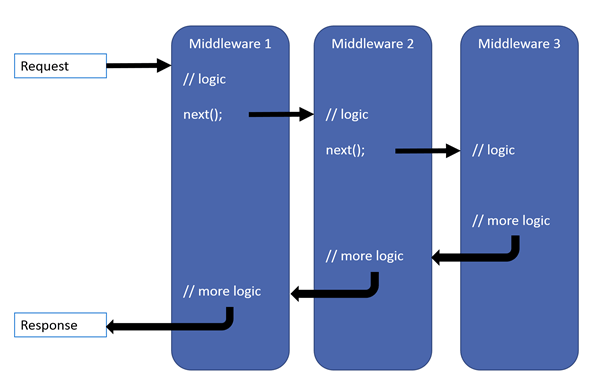
\includegraphics[width = 0.75\textwidth]{imgs/middleware.png}
    \caption{Схема конвейера запросов ASP.NET Core}
    \label{fig:Middleware}
\end{figure}

Таким образом, архитектура промежуточного ПО обеспечивает модульную и гибкую обработку HTTP-запросов, позволяя реализовывать в единой последовательности компонентов такие функции, как логирование, обработка ошибок и прочее.

\subsubsection{Встроенная поддержка DI(Dependency Injection)}
В ASP.NET Core есть встроенная поддержка внедрения зависимостей (Dependency Injection, DI). Она представляет собой механизм, обеспечивающий слабую связанность компонентов приложения и упрощающий управление зависимостями между ними. DI позволяет автоматически предоставлять необходимые объекты (сервисы) в классы, которые от них зависят, без необходимости создавать эти объекты вручную.

В ASP.NET Core внедрение зависимостей реализовано через встроенный контейнер служб, который управляет жизненным циклом и разрешением зависимостей. Сервисы регистрируются в контейнере, обычно в файле конфигурации приложения (например, Program.cs), с указанием времени их жизни --- Transient,  Scoped или Singleton. 

\begin{itemize}
	\item{Transient: Сервис создается при каждом запросе.}
	\item{Scoped: Сервис создается один раз для каждого запроса (подключения).}
	\item{Singleton: Сервис создается только один раз.}
\end{itemize}

При создании экземпляра класса, например контроллера, контейнер автоматически внедряет зарегистрированные зависимости через конструктор, что называется конструкторной инъекцией.
